%------------------------------------------------------------
%	PREAMBLE
%------------------------------------------------------------
\documentclass[12pt]{article}

\usepackage[english]{babel} % English language/hyphenation
\usepackage{amsmath,amsfonts,amsthm} % Math packages
\usepackage{graphicx}
\usepackage{natbib}
\usepackage{color}
\usepackage{url}
\usepackage{pdflscape}
\usepackage{caption}
\usepackage{subcaption}
\usepackage{setspace}
\usepackage[top=1.5in, bottom=1.5in, left=1in, right=1in]{geometry}
\usepackage{pbox}
\usepackage{bibentry}
\usepackage{hyperref}
\usepackage{longtable}
%\usepackage{subfigure}
\usepackage{appendix}
\usepackage{float}
\usepackage{tabularx}
\usepackage{amsmath,amsfonts,amsthm}
\usepackage{booktabs}
\usepackage{multirow}
\usepackage{adjustbox}
\usepackage{lscape}
\usepackage{changepage}
\usepackage{adjustbox}

\usepackage{lipsum}
\usepackage{hanging}

\usepackage[T1]{fontenc}
\usepackage[utf8]{inputenc}
\setlength{\parindent}{0em}

\newcommand{\numpy}{{\tt numpy}} % tt font for numpy

\topmargin -.5in
\textheight 9in
\oddsidemargin -.25in
\evensidemargin -.25in
\textwidth 7in
\linespread{1.40}

\begin{document}

\author{Stijn Vermeulen}
\title{Final project: Advanced Applied Econometrics \\ The Impact of Economic Policy on Reelection}
\maketitle

\section*{Disclaimer}
This paper was prepared for the course Advanced Applied Econometrics, taught at the Katholieke Universiteit Leuven in the year 2019. 
The goal of this project was to replicate and extend the results from the paper \textit{"How Do Budget Deficits and Economic Growth Affect 
Reelection Prospects? Evidence from a Large Panel of Countries"} by Adi Brender \& Allen Drazen (2008). The project focused mainly on the technical aspects of the paper and estimation process of a probit model in Stata. 
\pagebreak

\medskip
\section{Introduction}
The General Elections of 2018 in Italy has caused quite a stir in Europe as the elected government is set on an expansionary fiscal policy with the hope to improve its economic performance and gain popular support (CNBC, 2019). As economic policy is often mandated to governments, it is not surprising that governments and its incumbent leaders will try to use it to get reelected. With the 2008 article: \textit{How Do Budget Deficitis and Economic Growth Affect Reelection Prospects? Evidence from a Large Panel of Countries} Brender \& Drazen researched the effectiveness of economic policy on reelection prospects. In this article they used a logit model to study these effects and contributed to the literature on political business and budget cycles by explicitly distinguishing between developed and less developed countries. The aim of this paper is to replicate the author's results  and extend on it by implementing specification tests and computing the predicted margins and marginal effects.

\section{Data description}
The model in this paper will be estimated with the data used in the original paper of Brender \& Drazen (2008). The original dataset contained a total of 347 observations of election outcomes over the period 1960-2003 for 74 countries and included a variety of macroeconomic indicators and country characteristics. The relevant variables in this dataset can be categorized in three groups: the political variable, the macroeconomic performance variables and the institutional characteristics.\\  
The key political variable is the variable we are interested in to model: the reelection prospects of country leaders. REELECT is binary variable and will be either one, if the leader was reelected, or zero, if he was not. This paper uses the two samples of REELECT from Brender \& Drazen, each with its own definition of what is considered to be reelected. The \textit{Narrow sample} only contains observations where three conditions hold: 1) the leader had been in office for at least two budgetary years preceding the election year. 2) There was no legal limit on the leader's term 3) the leader stayed in office at least until one month before the elections. If he decided to leave office within one month before elections, REELECT is set at zero. The \textit{Expanded sample} extends the \textit{Narrow sample} by also including observations where: 4) the leader was replaced by a party member due to legal term limits or death. 5) the leader left office less than a year before elections and REELECT is set at zero in these instances. In our analysis, we will deviate from Brender \& Drazen and exclude all observations for Italy as these observations do no match the previous criteria (Governo Italiano, 2015).\\
The macroeconomic performance variables are the change in the government balance, both over the term and election year, and the GDP per capita growth rate (GDPPC\_gr) over the leader's term. Change in the government balance over the leader's term ($\Delta$GovBalance\_term) is constructed by the difference between the average balance of the two years preceding an election and the average balance of the two years preceding those. The change in balance for the election year ($\Delta$GovBalance\_ey) is constructed similarly by taking the difference of the balance in the election year and the previous year. Both variables are straightforward to interpret: a positive number implies an improvement in the balance relative to before and vice versa.\\
The last category of variables used in this paper are the institutional variables: New Democracy, Development level and Majoritarian Electoral System. All three are dummy variables. A country is considered a new democracy for 4 elections after it changed form a negative to positive \textit{polity} value in POLITY IV database. The variable Developed is set at one if a country was part of the OECD over the entire sample period and zero if otherwise. The last variable Majoritarian describes whether the leader was voted through a system based on the majority of votes. An example of a country with a Majoritarian voting system would be the United States.\\

\section{Model}
To test whether changes in the government balance or growth have any effect on a leader's reelection prospect, we'll be estimating a probit model. The probit model is a non-linear, binary response model which ensures that the estimated response probability will be strictly between zero and one. The advantage of choosing the probit model over the logit model, as was done in Brender \& Drazen (2008), lies in the assumption of the standard normal distribution of the residuals. This assumption will facilitate the analysis of the specification tests, which will be discussed later on (Wooldridge, 2013, p586). \\
\begin{table}
 \centering
 \caption{\small{Probit Model - The Effects of Budget Balances and Growth on the Probability of Reelection}}
 \label{table:probit}
\begin{adjustbox}{width=1\textwidth}
\begin{tabular}{l*{6}{c}}
\hline\hline \\[-0.5em]

Dependent variable: & \multicolumn{3}{c}{\textbf{Narrow Sample}} & \multicolumn{3}{c}{\textbf{Expanded Sample}} \\ 
		\cmidrule(l){2-4} \cmidrule(l){5-7} 
		
 \textbf{REELECT} &\multicolumn{1}{c}{(1)}&\multicolumn{1}{c}{(2)}&\multicolumn{1}{c}{(3)}&\multicolumn{1}{c}{(4)}&\multicolumn{1}{c}{(5)}&\multicolumn{1}{c}{(6)}\\
 &\multicolumn{1}{c}{All countries}&\multicolumn{1}{c}{Developed}&\multicolumn{1}{c}{Less Developed}&\multicolumn{1}{c}{All countries}&\multicolumn{1}{c}{Developed}&\multicolumn{1}{c}{Less Developed}\\
\hline
 & & & & & & \\
$\Delta$ \textbf{GovBalance\_term}  &       8.165\sym{**} &       11.47\sym{**} &       9.702         &       6.157\sym{*}  &       7.219         &       8.159\sym{*}  \\
            &      (1.99)         &      (2.22)         &      (1.29)         &      (1.95)         &      (1.59)         &      (1.72)         \\

$\Delta$ \textbf{GovBalance\_ey}      &       8.341\sym{*}  &       24.26\sym{***}&      -2.362         &       6.630\sym{*}  &       21.42\sym{***}&       0.458         \\
            &      (1.81)         &      (3.41)         &     (-0.35)         &      (1.69)         &      (3.25)         &      (0.09)         \\

\textbf{GDPPC}\textsubscript{gr}  &       10.92\sym{**} &      -3.182         &       23.02\sym{***}&  13.54\sym{***}&     -0.0730         &       21.12\sym{***}   \\
            &      (2.57)         &     (-0.51)         &      (3.33)         &      (3.75)         &     (-0.01)         &      (4.12)        \\

\textbf{New Democracies}       &       0.409\sym{*}  &       0.701         &       0.382         &       0.207         &       0.758\sym{*}  &       0.126         \\
            &      (1.75)         &      (1.57)         &      (1.32)         &      (1.11)         &      (1.72)         &      (0.59)         \\

\textbf{Developed Countries}     &       0.520\sym{**} &                     &                     &       0.457\sym{***}&                     &                     \\
            &      (2.39)         &                     &                     &      (2.64)         &                     &                     \\


\textbf{Maj. Electoral System}    &       0.451\sym{**} &       0.373         &       0.476\sym{*}  &       0.425\sym{***}&       0.327         &       0.425\sym{*}  \\
            &      (2.35)         &      (1.40)         &      (1.65)         &      (2.61)         &      (1.36)         &      (1.87)         \\

\textbf{Constant}      &      -0.808\sym{***}&       0.101         &      -1.202\sym{***}&      -0.901\sym{***}&     -0.0860         &      -1.073\sym{***}\\
            &     (-3.22)         &      (0.48)         &     (-3.50)         &     (-4.76)         &     (-0.43)         &     (-4.69)         \\
\hline
\(N\)       &         249         &         158         &          91         &         341         &         174         &         167         \\
 LM test statistic & 0.9826               & 21.3991             & 30.5473               & 1.7455               & 46.5495             & 23.0553               \\
 with p-values & (0.6112) & (2.255e-5)          & (2.327e-7) & (0.4178) & (7.797e-11)         & (9.854e-6) \\
 \hline\hline
\multicolumn{7}{l}{\footnotesize \textit{t} statistics in parentheses; \sym{*} \(p<.10\), \sym{**} \(p<.05\), \sym{***} \(p<.01\)
}\\
\end{tabular}
\end{adjustbox}

\end{table}\\
In Table \ref{table:probit} the results of the regular probit are reported. The same set-up is used as in the original author's paper: REELECT is used as the dependent variable and $\Delta$GovBalance\_term, $\Delta$GovBalance\_ey, GDPPC\_gr, New Democracies, Developed Countries, Maj. Electoral System are the regressors. The regression is run for both the \textit{Narrow} and \textit{Expanded Sample} and each sample is divided separately in a Complete, Developed and Less Developed set.\\

The results from the probit model in Table \ref{table:probit} are a replication of the original regression run by Brender \& Drazen. Both in the \textit{Narrow} and \textit{Expanded sample} the macroeconomic variables prove to be significant, albeit with a varying degree of significance level. The positive signs of the macroeconomic variables also imply that voters reward leaders who improve the government balance or growth rate and punish those that worsen economic performance. When only Developed or Less Developed countries are taken into consideration, the results change slightly. For Developed countries, the significance of growth disappears implying more emphasis is put on the government balance when people are making their vote. For Less Developed countries, the reverse is true as no significance is found for the fiscal variables and growth plays a bigger role in reelection prospects.\\
While the probit model allows us to estimate a prediction of the probability of reelection, a shortcoming of the model is that it will be inconsistent when incorrectly specified. If we want to be sure our model is correctly specified, we have to impose two specification tests: a test for heteroskedasticity of the residuals and a test for normality of the residuals. \\

\textbf{Heteroskedasticity}\\
The regular probit model assumes that the residuals $\epsilon$ is homoskedastic, i.e. the variance is constant (Verbeek, 2004, p16). If this assumption does not hold, the probit estimation will break down and lead to inconsistent results. Since the model uses data from a large variety of countries with heterogeneity, is it not unreasonable to assume that the homoskedasticity condition might be violated. Therefore, if we want to make sure heteroskedasticity isn't a problem, we have to impose a specification test on the model.\\
To test for heteroskedasticity, we will use the likelihood ratio (LR) test to check whether the difference between the likelihood function of a model where we allow for heteroskedasticity and the regular probit model is significantly different from zero. The identification of the heteroskedastic variables involves two steps. First, all variables are included separately in the model as potential cause of the heteroskedasticity. This process is done for each of the original equations and only the variables that reject the null of the LR test at the 10\% significance level are kept as heteroskedastic variables. If more than one variable rejects the null, all variables who reject it will be included as heteroskedastic.\\\pagebreak

Table \ref{table:hetprobit} presents the results from the probit model adjusted for heteroskedasticity. The original six equations are tested for heteroskedasticity and all reject the null of homoskedasticity with at least one variable as heteroskedastic. The heteroskedastic variables are marked by a $\circ$ and the p-values of the LR test are included in the bottom row of the table.\\
When we compare the results from the regular probit with the hetprobit, the difference is most apparent in the \textit{Narrow sample}. All regressors in equation 1 with all countries and equation 3 with only the Less Developed countries lose their significance. In equation 2, the only significant variables turn out to be $\Delta$GovBalance\_ey, GDPPC\_gr and New Democracies. An especially curious outcome is the negative value of GDPPC\_gr which implies that voters punish higher growth rates. If we make the comparison in the \textit{Expanded sample}, the difference with the regular probit is less pronounced. Significance remains roughly the same, albeit with a difference in the level. A noteworthy difference is that similarly to the \textit{Narrow sample} the growth rate gets a significant negative coefficient.\\

Overall, we can conclude that the homoskedasticity assumption does not hold in the original probit model and, therefore, should be corrected for by using a hetprobit model. When we adjust the model for heteroskedasticity, the results change more so in the \textit{Narrow} than the \textit{Expanded sample}. \\

\textbf{Normality}\\
A second assumption that needs to hold in a probit regression is the normality of the residuals. If the residuals do not have a normal distribution, the model is incorrectly specified and this leads to inconsistent results. Therefore, we will impose a Lagrange Multiplier (LM) specification test this assumption. This test will be imposed on both the regular probit and hetprobit model.\\
To test the normality assumption, we follow the process described by Verbeek (2004, p201-202) and construct an auxiliary regression to compute the LM test statistic. This auxiliary regression is a regression of ones upon $\widehat{\epsilon}\textsubscript{i}^Gx^\prime\textsubscript{i},\widehat{\epsilon}\textsubscript{i}^G(x^\prime\textsubscript{i}\widehat{\beta})^2$ and $ \widehat{\epsilon}\textsubscript{i}^G(x^\prime\textsubscript{i}\widehat{\beta)}^3$ with $\widehat{\epsilon}\textsubscript{i}^G$ the generalized residuals and $x\textsubscript{i}$ the vector of variables in the orignal model. Once this regression is completed, we can compute the LM statistic by multiplying the $R^2$ wit the number of observations N and test it for the null hypothesis of normality. The statistics of all equations for both the probit and hetprobit model are reported in Table \ref{table:lm}.\\
\begin{table}[H]
 \centering
  \caption{\small{Probit Model adjusted for heteroskedasticity - The Effects of Budget Balances and Growth on the Probability of Reelection}}
 \label{table:hetprobit}
\begin{adjustbox}{width=\textwidth}
\begin{tabular}{l*{6}{c}} 
\hline\hline \\[-0.5em]

Dependent variable: & \multicolumn{3}{c}{\textbf{Narrow Sample}} & \multicolumn{3}{c}{\textbf{Expanded Sample}} \\ 
		\cmidrule(l){2-4} \cmidrule(l){5-7} 
		
 \textbf{REELECT} &\multicolumn{1}{c}{(1)}&\multicolumn{1}{c}{(2)}&\multicolumn{1}{c}{(3)}&\multicolumn{1}{c}{(4)}&\multicolumn{1}{c}{(5)}&\multicolumn{1}{c}{(6)}\\
 &\multicolumn{1}{c}{All countries}&\multicolumn{1}{c}{Developed}&\multicolumn{1}{c}{Less Developed}&\multicolumn{1}{c}{All countries}&\multicolumn{1}{c}{Developed}&\multicolumn{1}{c}{Less Developed}\\
\hline
 & & & & & & \\
$\Delta$ \textbf{GovBalance\_term} & 30.58 & ^\circ5.735 & 4.735 & 14.56\sym{*} & 5.700 & 12.25 \\
 & (1.30) & (1.34) & (0.70) & (1.80) & (1.30) & (1.41) \\

$\Delta$ \textbf{GovBalance\_ey} & ^\circ21.70 & 17.84\sym{**} & ^\circ9.144 & ^\circ21.13\sym{**} & 18.08\sym{***}& ^\circ10.77 \\
 & (1.04) & (2.12) & (0.69) & (1.97) & (2.69) & (1.03) \\

\textbf{GDPPC}\textsubscript{gr} & ^\circ37.63 & -6.593\sym{**} & 9.228 & ^\circ17.20\sym{*} & -6.619\sym{**} & ^\circ27.48\sym{***}\\
 & (1.44) & (-1.98) & (0.75) & (1.65) & (-2.22) & (2.91) \\

\textbf{New Democracies}& 2.370 & ^\circ0.428\sym{**} & 0.222 & 0.798 & ^\circ0.514\sym{***}& 0.231 \\
 & (1.40) & (1.97) & (0.66) & (1.50) & (2.67) & (0.66) \\

\textbf{Developed Countries}  & 3.167 & & & 1.447\sym{**} & & \\
 & (1.26) & & & (2.25) & & \\

\textbf{Maj. Electoral System} & 1.478 & 0.192 & 0.171 & 0.802\sym{*} & 0.273 & 0.696\sym{*} \\
 & (1.18) & (0.86) & (0.54) & (1.94) & (1.16) & (1.78) \\


\textbf{Constant}& -3.480 & 0.172 & -0.520 & -1.828\sym{***}& 0.0918 & -1.389\sym{***}\\
 & (-1.58) & (1.37) & (-0.67) & (-3.06) & (0.67) & (-3.56) \\ [0.5em]
\hline 
\(N\) & 249 & 158 & 91 & 341 & 174 & 167 \\
p-value LR test         &   5.56e-5         &    6.48e-4         &      0.0137         &     1.19e-3        &     3.91e-3         &      0.0705         \\
LM test statitistic & 43.5201              & 20.8386             & 13.3731               & 23.3589              & 44.8822             & 39.50427              \\
with p-values & (3.546e-10)          & (2.985e-5)          & (1.248e-3)            & (8.466e-5)           & (1.795e-10)         & (2.641e-9)\\
\hline\hline
\multicolumn{7}{l}{\footnotesize \textit{t} statistics in parentheses; \sym{*} \(p<.10\), \sym{**} \(p<.05\), \sym{***} \(p<.01\); Heteroskedastic Variables marked with ^\circ}\\

\end{tabular}
\end{adjustbox}


\end{table}\\
The test statistics from Table \ref{table:lm} are reported together with either their p-values in round brackets or bootstrapped 95\% confidence interval (CI) in square brackets. Based on this we can conclude that only equation 1, 3 and 6 of the regular probit model pass the normality test. All other equations reject the null hypothesis. It should be noted, however, that the Lagrange Multiplier test is only asymptotically consistent. Therefore, only for the equations with bootstrapped CIs can we safely make a conclusion on normality of the residuals. The computation of the bootstrapped CIs for the other equations was not possible as it either led to non-convergence of the likelihood function or there were not enough observations available. It is possible that either one of these equations does pass the normality test, however, no safe answer can be given with the current information.\\ 
\begin{table}[H]

\caption{\small{Normality test - Lagrange Multiplier test statistic}}
 \label{table:lm}
\begin{adjustbox}{width=\textwidth}
\begin{tabular}{ccccccc}
\hline\hline
 & & &&&&&
\mediumlarge{\textbf{LM Statistic}               & \textbf{Equation 1}  & \textbf{Equation 2} & \textbf{Equation 3}   & \textbf{Equation 4}  & \textbf{Equation 5} & \textbf{Equation 6}}   \\  [1em]
\hline 
&&&&&&&
\multirow{2}{*}{\textbf{Probit}}    & 0.9826               & 21.3991             & 30.5473               & 1.7455               & 46.5495             & 23.0553               \\
                                    & {[}0.115 , 17.787{]} & (2.255e-5)          & {[}14.454 , 62.128{]} & {[}3.735 , 25.980{]} & (7.797e-11)         & {[}14.454 , 62.128{]} \\
                                    [1em]
\multirow{2}{*}{\textbf{Hetprobit}} & 43.5201              & 20.8386             & 13.3731               & 23.3589              & 44.8822             & 39.50427              \\
                                    & (3.546e-10)          & (2.985e-5)          & (1.248e-3)            & (8.466e-5)           & (1.795e-10)         & (2.641e-9)\\
[0.5em]
\hline\hline
\multicolumn{7}{l}{\footnotesize Where available bootstrapped confidence intervals in square brackets and p-values in round brackets}\\
\end{tabular}
\end{adjustbox}
\end{table}\\

\textbf{Model predictions and marginal effects}\\
A last extension to the original Brender \& Drazen paper we will discuss here, is a more detailed analysis of the model predictions and marginal effects.This was only briefly touched upon in the original paper, yet it may be useful when we want to give policy advice.\\
Since the probit and hetprobit are non-linear models, the marginal effects will no longer be constant and will differ in value across its own range. How the model predictions and marginal effects differ are presented in Figure \ref{Predicted_Narrow} and Figure \ref{Predicted_Expanded}. Both figures are plotted using only the main equations 1 and 4. Both the probit (full lines) and hetprobit model (dashed lines) are included and the figures also make a distinction between developed (blue \& orange) and less developed countries (green \& red).\\
Figure \ref{Predicted_Narrow}  presents the predicted margins or model predictions for all the macroeconomic variables both in the \textit{Narrow} (upper panel) and \textit{Expanded sample} (lower panel). Starting our analysis with the regular probit model, we can make two general observations: first, in both samples all three variables show an increasing trend in probability of reelection implying better outcomes lead to better reelection prospects. Second, the reelection prospects are higher in developed compared to less developed countries.\\

\begin{figure}[H]
    \centering
    \label{figure:margins}
    \begin{subfigure}[H]{1\textwidth}
    \centering
    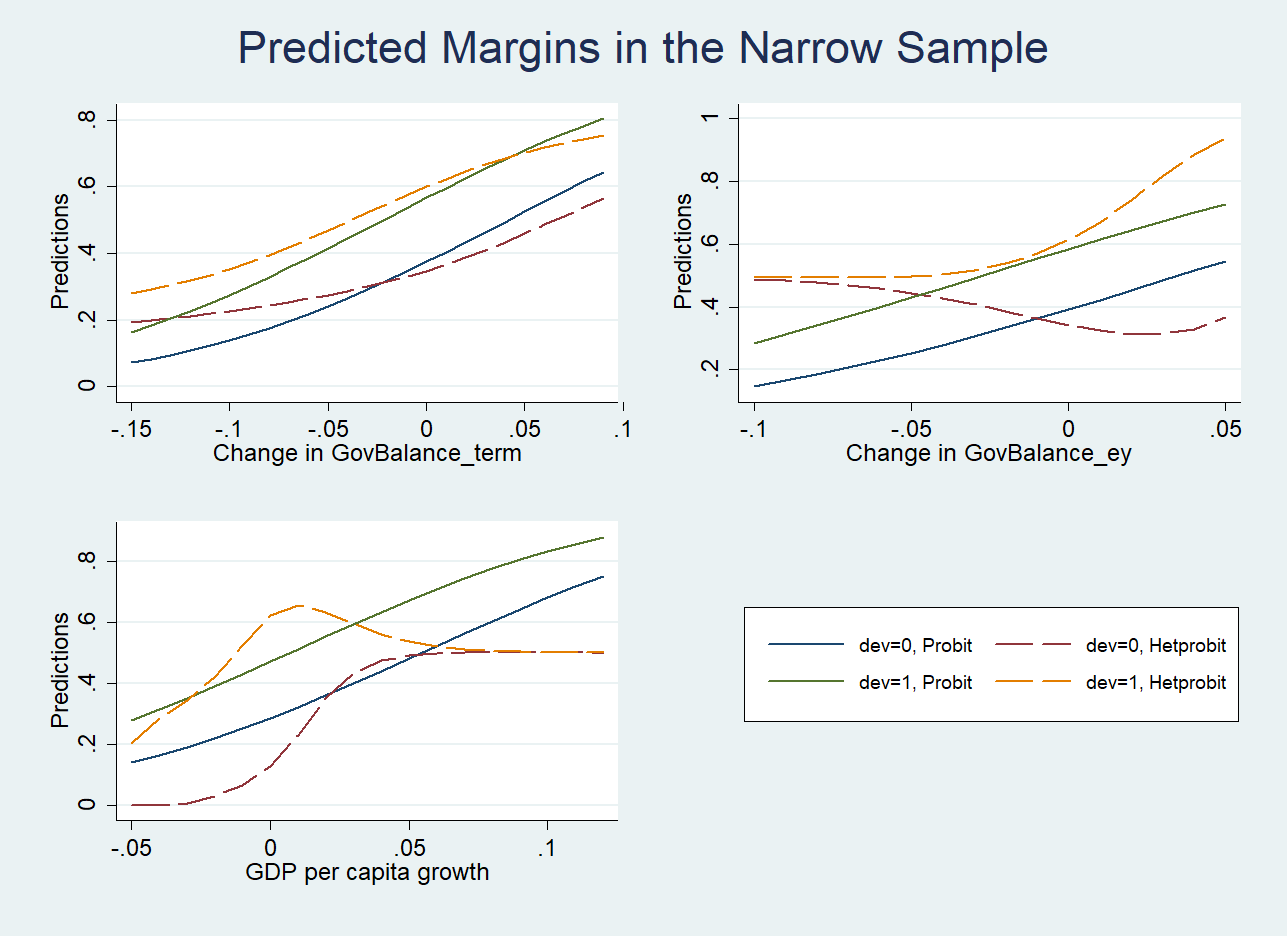
\includegraphics[width=0.8\textwidth]{Predicted_Narrow.png}
    \end{subfigure}
    \begin{subfigure}[H]{1\textwidth}
    \centering
    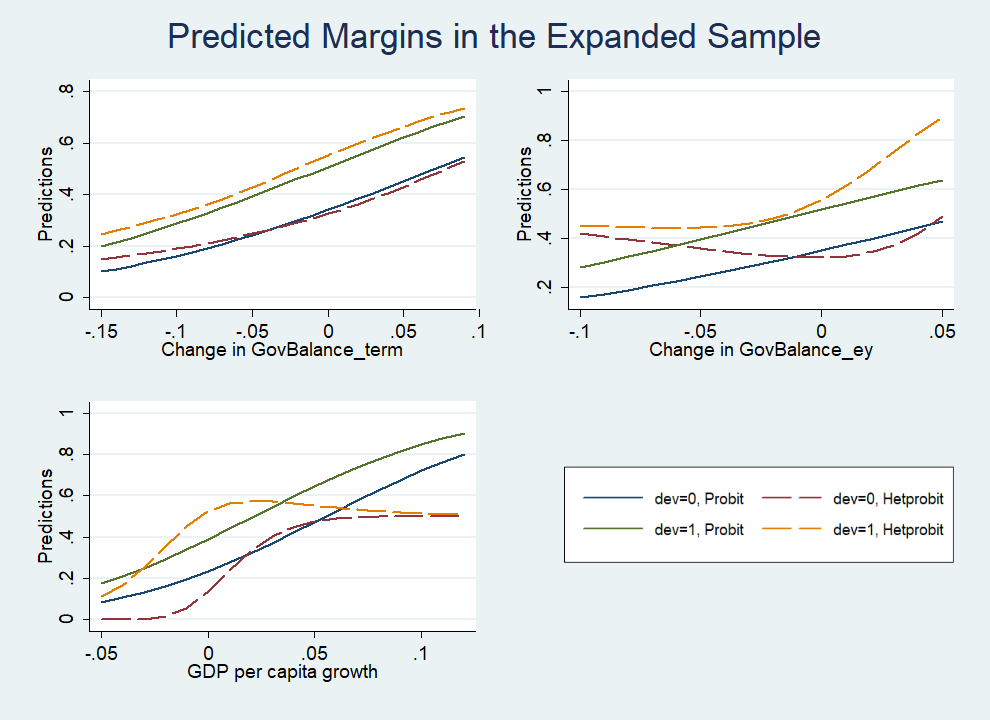
\includegraphics[width=0.8\textwidth]{Predicted_Expanded.png}
    \end{subfigure}
    \caption{\small{Predicted margins of the regular Probit (solid lines) and Heteroskedastic Probit model (dashed lines) for both Developed and Less Developed countries. Variables displayed are: the change in Government Balance over the leader's term, change in Government Balance in the election year and GDP per capita growth rate}}
    \label{Predicted_Narrow}
\end{figure}
\begin{figure}[H]
    \centering
    \label{figure:marginal effects}
        \begin{subfigure}[H]{1\textwidth}
    \centering
    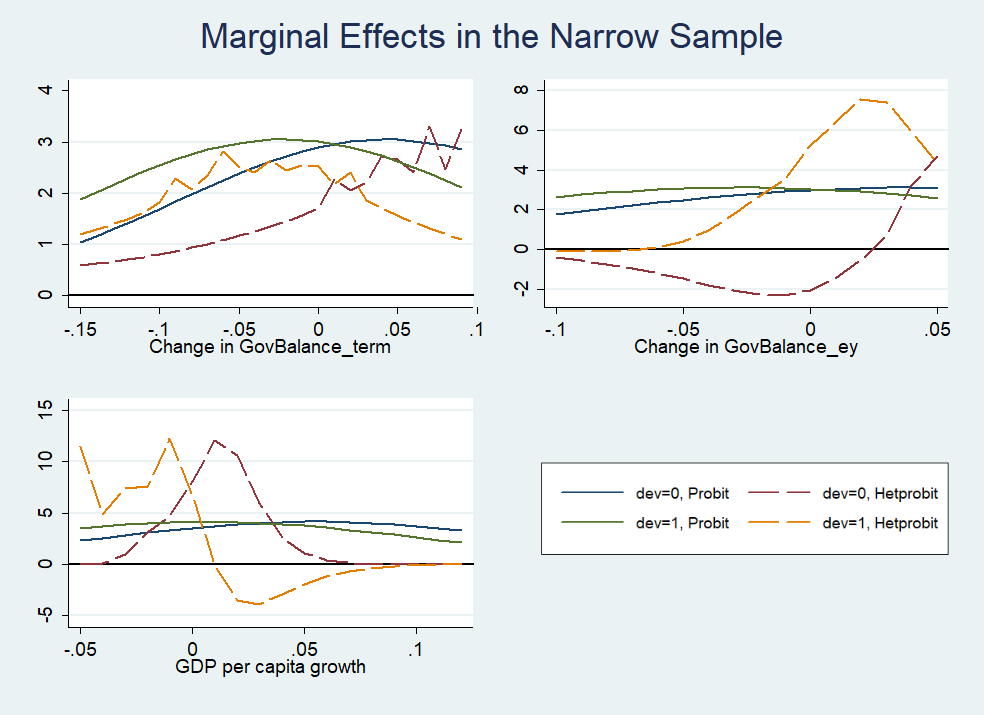
\includegraphics[width=0.8\textwidth]{AME_Narrow.png}
    \end{subfigure}
    \begin{subfigure}[H]{1\textwidth}
    \centering
    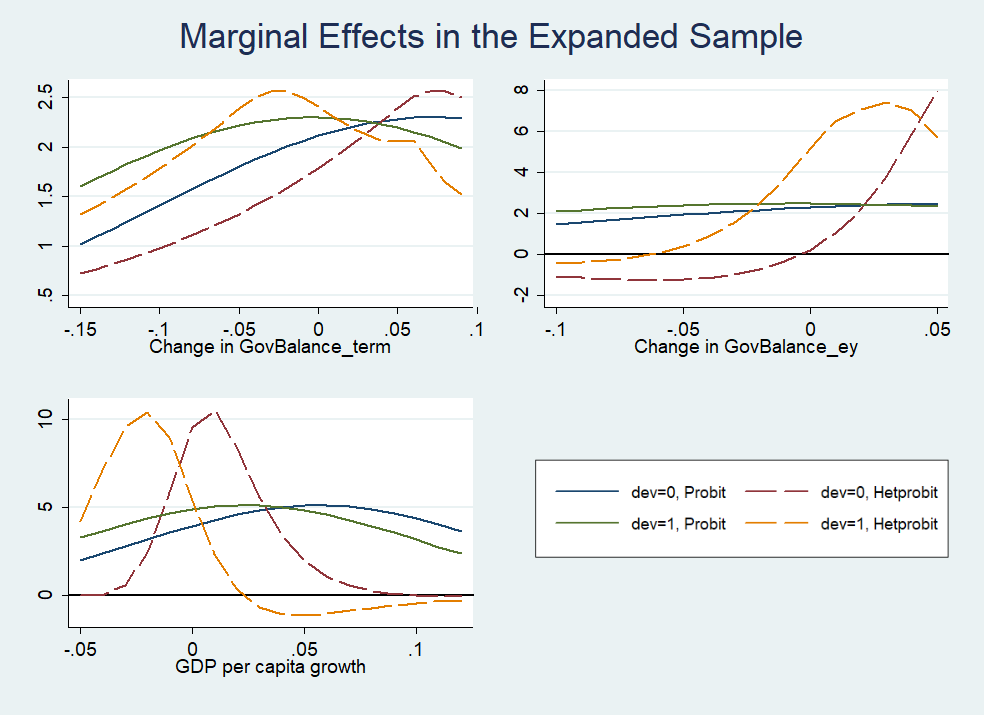
\includegraphics[width=0.8\textwidth]{AME_expanded.png}
    \end{subfigure}
    \caption{\small{Average marginal effects of the regular Probit (solid lines) and Heteroskedastic Probit model (dashed lines) for both Developed and Less Developed countries. Variables displayed are: the change in Government Balance over the leader's term, change in Government Balance in the election year and GDP per capita growth rate}}
    \label{Predicted_Expanded}
\end{figure}
\\
When we consider the results from the hetprobit model, however, we have to slightly adjust our conclusion. In particular, the change in government balance in the election year shows a negative trend for less developed countries. The third variable, GDP per capita growth, also shows a negative trend after reaching its peak at $\pm$ 0.01\%. These negative trends are present in both the \textit{Narrow} and \textit{Expanded sample}, though in the latter it is less pronounced.\\
Figure \ref{Predicted_Expanded} plots the first derivatives of the plots of Figure \ref{Predicted_Narrow} and gives us a better picture where a change of a variable will have the largest effect on reelection prospects. Once more, we can make some general conclusions: first, the marginal effects of developed countries are higher for negative values of the variables compared to less developed countries. Second, almost all plots are non-constant which implies changes in reelection prospects differ depending on each scenario one might find itself in, e.g. the effect of an improvement of the government balance in the election year from -0.05 to -0.04 differs from 0.04 to 0.05.\\   
\section{Conclusion}
The aim of this paper was to replicate and to extend on the original article written by Brender \& Drazen (2008) and to further our understanding of the effectiveness of using macroeconomic variables for reelection purposes. The original logit model is substituted for a probit model and two specification tests are imposed to verify whether the model is correctly specified. We find evidence of heteroskedasticity in all of the authors' original regression equations and only 3 out of the 6 original equations pass the normality test. In addition, this paper also extends the orignal article by looking at the predicted margins and marginal effects and finds that, with a few exceptions, improvements in the macroeconomic variables lead to higher reelection prospects. 
\pagebreak
\section{References}
\item Brender, A., Drazen, A. (2008), How do budget deficits and economic growth affect reelection prospects? Evidence from a large panel of countries, \textit{American Economic Review}, 98 (5), pp. 2203-20.
\item CNBC. (2019, May 28). Italy vs the EU: Markets spooked as Europe prepares for another budget showdown. Retrieved May 29, 2019, from https://www.cnbc.com/2019/05/28/italy-vs-the-eu-markets-spooked-as-europe-awaits-budget-showdown.html
\item Governo Italiano, Presidenza del Consiglio dei Ministri. (2015, November 9). I Governi dal 1943 ad oggi. Retrieved May 28, 2019, from {http://www.governo.it/i-governi-dal-1943-ad-oggi/191?fbclid\=IwAR1\\
9TRl3rVlONUm8gU3oTYHz37TZ5txVn6hdr0T80iQDvGyQ5SSEDKoQG34}
\item Verbeek, M. (2004). A Guide to Modern Econometrics (2nd ed.). Retrieved from \\https://thenigerianprofessionalaccountant.files.wordpress.com/2013/04/modern-econometrics.pdf
\item Wooldridge, J. M. (2013). Introductory Econometrics: A Modern Approach (5th ed.). South-Western, Mason, OH 45040 USA: Cengage Learning.


\end{document}